\adjustbox{valign=t}{
\begin{minipage}[t]{.5\linewidth}
  1. \textit{min-heap} \\[1em]
  \adjustbox{valign=t}{
    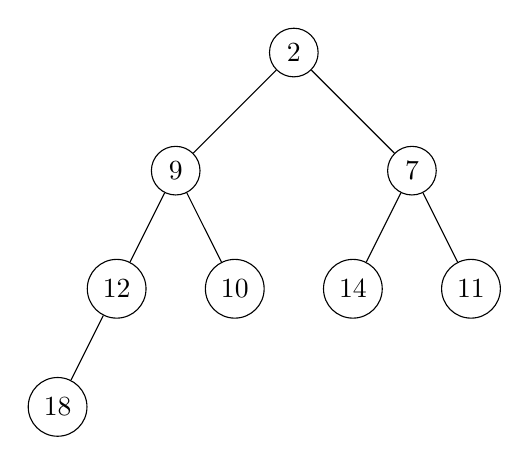
\begin{tikzpicture}
      \node[circle,draw](z){$2$}
        child{
          node[circle,draw]{$9$}
          child {
            node[circle,draw]{$12$}
            child { 
              node[circle,draw]{$18$}
            }
            child[missing] { }
          }
          child {
            node[circle,draw]{$10$}
          }
        }
        child[missing] { }
        child{
          node[circle,draw]{$7$}
          child {
            node[circle,draw]{$14$}
          }
          child {
            node[circle,draw]{$11$}
          }
        };
    \end{tikzpicture}
  }
\end{minipage}
}
\adjustbox{valign=t}{
\begin{minipage}[t]{.5\linewidth}
  2. \textit{Step 1} \\[1em]
  \adjustbox{valign=t}{
    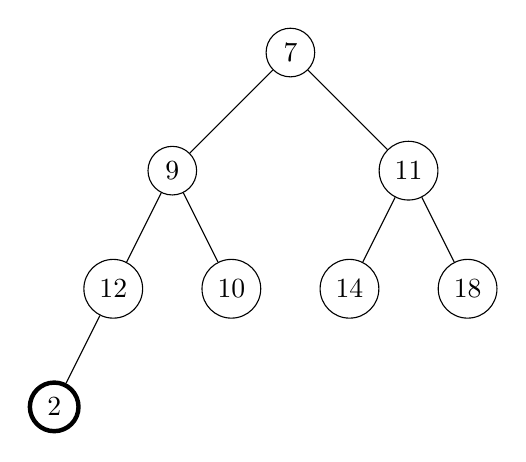
\begin{tikzpicture}
      \node[circle,draw](z){$7$}
        child{
          node[circle,draw]{$9$}
          child {
            node[circle,draw]{$12$}
            child { 
              node[circle,line width=1.6pt,draw]{$2$}
            }
            child[missing] { }
          }
          child {
            node[circle,draw]{$10$}
          }
        }
        child[missing] { }
        child{
          node[circle,draw]{$11$}
          child {
            node[circle,draw]{$14$}
          }
          child {
            node[circle,draw]{$18$}
          }
        };
    \end{tikzpicture}
  }
\end{minipage}
} \\[2em]

\adjustbox{valign=t}{
\begin{minipage}[t]{.5\linewidth}
  3. \textit{Step 2} \\[1em]
  \adjustbox{valign=t}{
    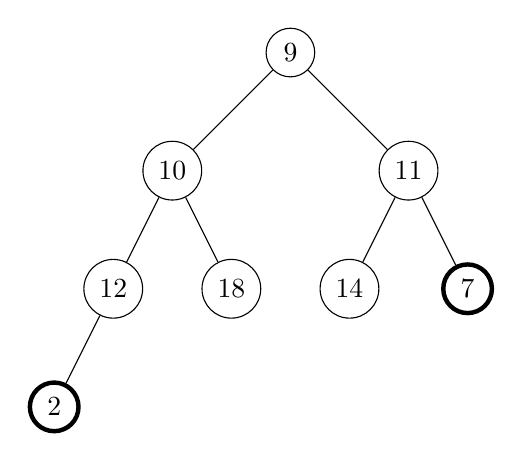
\begin{tikzpicture}
      \node[circle,draw](z){$9$}
        child{
          node[circle,draw]{$10$}
          child {
            node[circle,draw]{$12$}
            child { 
              node[circle,line width=1.6pt,draw]{$2$}
            }
            child[missing] { }
          }
          child {
            node[circle,draw]{$18$}
          }
        }
        child[missing] { }
        child{
          node[circle,draw]{$11$}
          child {
            node[circle,draw]{$14$}
          }
          child {
            node[circle,line width=1.6pt,draw]{$7$}
          }
        };
    \end{tikzpicture}
  }
\end{minipage}
}
\adjustbox{valign=t}{
\begin{minipage}[t]{.5\linewidth}
  4. \textit{Step 3} \\[1em]
  \adjustbox{valign=t}{
    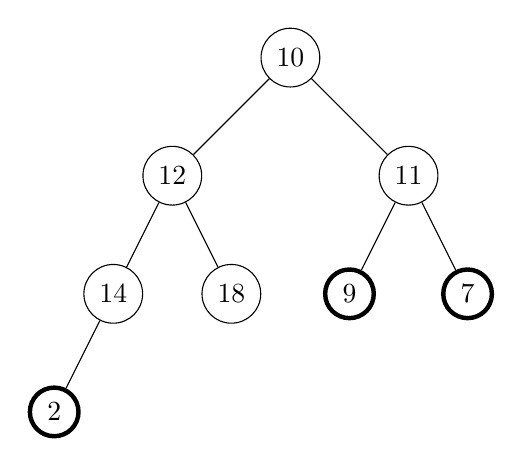
\begin{tikzpicture}
      \node[circle,draw](z){$10$}
        child{
          node[circle,draw]{$12$}
          child {
            node[circle,draw]{$14$}
            child { 
              node[circle,line width=1.6pt,draw]{$2$}
            }
            child[missing] { }
          }
          child {
            node[circle,draw]{$18$}
          }
        }
        child[missing] { }
        child{
          node[circle,draw]{$11$}
          child {
            node[circle,line width=1.6pt,draw]{$9$}
          }
          child {
            node[circle,line width=1.6pt,draw]{$7$}
          }
        };
    \end{tikzpicture}
  }
\end{minipage}
} \\[2em]

\adjustbox{valign=t}{
\begin{minipage}[t]{.5\linewidth}
  5. \textit{Step 4} \\[1em]
  \adjustbox{valign=t}{
    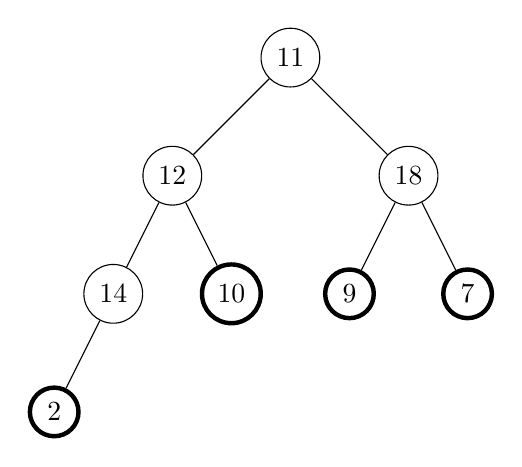
\begin{tikzpicture}
      \node[circle,draw](z){$11$}
        child{
          node[circle,draw]{$12$}
          child {
            node[circle,draw]{$14$}
            child { 
              node[circle,line width=1.6pt,draw]{$2$}
            }
            child[missing] { }
          }
          child {
            node[circle,line width=1.6pt,draw]{$10$}
          }
        }
        child[missing] { }
        child{
          node[circle,draw]{$18$}
          child {
            node[circle,line width=1.6pt,draw]{$9$}
          }
          child {
            node[circle,line width=1.6pt,draw]{$7$}
          }
        };
    \end{tikzpicture}
  }
\end{minipage}
}
\adjustbox{valign=t}{
\begin{minipage}[t]{.5\linewidth}
  6. \textit{Step 5} \\[1em]
  \adjustbox{valign=t}{
    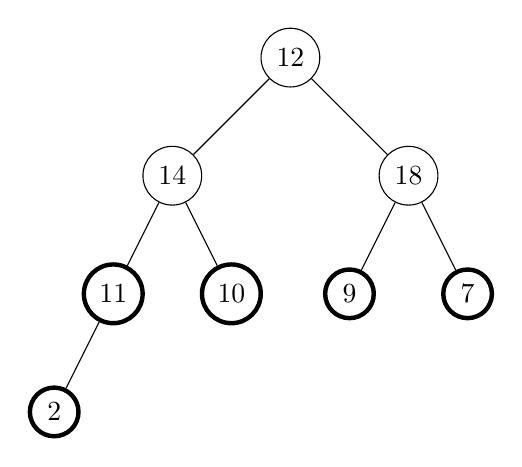
\begin{tikzpicture}
      \node[circle,draw](z){$12$}
        child{
          node[circle,draw]{$14$}
          child {
            node[circle,line width=1.6pt,draw]{$11$}
            child { 
              node[circle,line width=1.6pt,draw]{$2$}
            }
            child[missing] { }
          }
          child {
            node[circle,line width=1.6pt,draw]{$10$}
          }
        }
        child[missing] { }
        child{
          node[circle,draw]{$18$}
          child {
            node[circle,line width=1.6pt,draw]{$9$}
          }
          child {
            node[circle,line width=1.6pt,draw]{$7$}
          }
        };
    \end{tikzpicture}
  }
\end{minipage}
} \\[2em]

\adjustbox{valign=t}{
\begin{minipage}[t]{.5\linewidth}
  7. \textit{Step 6} \\[1em]
  \adjustbox{valign=t}{
    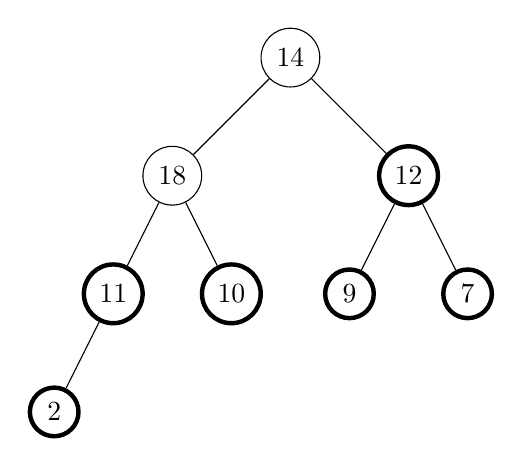
\begin{tikzpicture}
      \node[circle,draw](z){$14$}
        child{
          node[circle,draw]{$18$}
          child {
            node[circle,line width=1.6pt,draw]{$11$}
            child { 
              node[circle,line width=1.6pt,draw]{$2$}
            }
            child[missing] { }
          }
          child {
            node[circle,line width=1.6pt,draw]{$10$}
          }
        }
        child[missing] { }
        child{
          node[circle,line width=1.6pt,draw]{$12$}
          child {
            node[circle,line width=1.6pt,draw]{$9$}
          }
          child {
            node[circle,line width=1.6pt,draw]{$7$}
          }
        };
    \end{tikzpicture}
  }
\end{minipage}
}
\adjustbox{valign=t}{
\begin{minipage}[t]{.5\linewidth}
  8. \textit{Step 7} \\[1em]
  \adjustbox{valign=t}{
    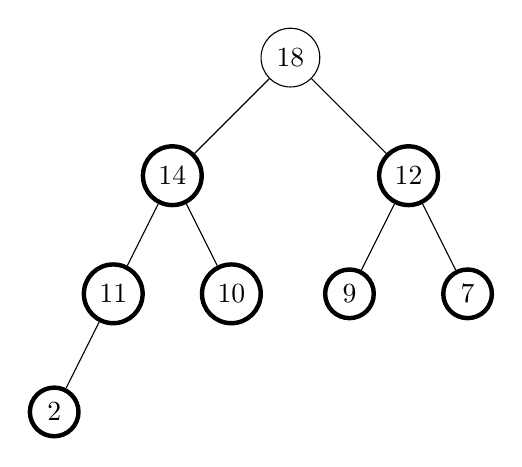
\begin{tikzpicture}
      \node[circle,draw](z){$18$}
        child{
          node[circle,line width=1.6pt,draw]{$14$}
          child {
            node[circle,line width=1.6pt,draw]{$11$}
            child { 
              node[circle,line width=1.6pt,draw]{$2$}
            }
            child[missing] { }
          }
          child {
            node[circle,line width=1.6pt,draw]{$10$}
          }
        }
        child[missing] { }
        child{
          node[circle,line width=1.6pt,draw]{$12$}
          child {
            node[circle,line width=1.6pt,draw]{$9$}
          }
          child {
            node[circle,line width=1.6pt,draw]{$7$}
          }
        };
    \end{tikzpicture}
  }
\end{minipage}
} \\[2em]

\adjustbox{valign=t}{
\begin{minipage}[t]{.5\linewidth}
  9. \textit{Step 8 (sorted)} \\[1em]
  \adjustbox{valign=t}{
    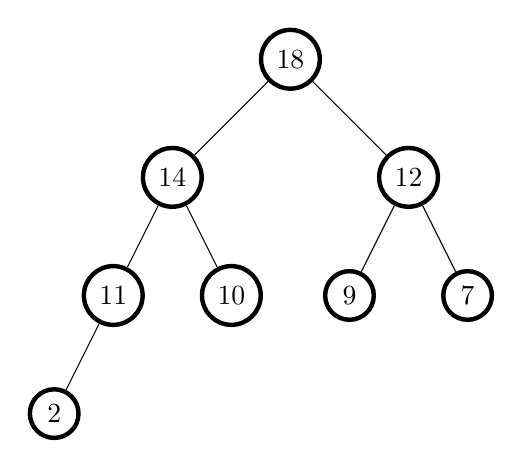
\begin{tikzpicture}
      \node[circle,line width=1.6pt,draw](z){$18$}
        child{
          node[circle,line width=1.6pt,draw]{$14$}
          child {
            node[circle,line width=1.6pt,draw]{$11$}
            child { 
              node[circle,line width=1.6pt,draw]{$2$}
            }
            child[missing] { }
          }
          child {
            node[circle,line width=1.6pt,draw]{$10$}
          }
        }
        child[missing] { }
        child{
          node[circle,line width=1.6pt,draw]{$12$}
          child {
            node[circle,line width=1.6pt,draw]{$9$}
          }
          child {
            node[circle,line width=1.6pt,draw]{$7$}
          }
        };
    \end{tikzpicture}
  }
\end{minipage}
} \\